% !TeX root = ../main.tex
\chapter{Control System and ROS 2 Integration}
\label{chap:controls}

\label{sec:control-architecture}
The crawler requires a common software interface for operator commands, wheel actuation, camera viewing, and planned inertial and pressure measurements. Robot Operating System 2 (ROS 2) organizes these functions as communicating nodes. Nodes can exchange data within one computer or across a network, and typed messages define the interfaces between them \citep{ros2JazzyNodes,ros2JazzyInterfaces}. For this project, that organization allows joystick processing, motor communication, and camera acquisition to be developed and checked separately while remaining accessible to the operator station.

The integration uses ROS 2 Jazzy and the packages in the author's \texttt{vacuum\_crawler} repository. This chapter describes revision \texttt{75dc509}, reviewed on November 12, 2026 \citep{hernandezVacuumCrawler2026}. The command path connects the standard joystick driver to the project's teleoperation node, then branches to the wheel controller and Teensy camera-servo bridge. Camera nodes provide visual feedback through a separate path. The intended architecture also includes an inertial measurement unit (IMU), pressure sensing, and three-dimensional (3D) camera feedback. 

ROS 2 is selected as an integration framework rather than as evidence of autonomous operation or closed-loop motion control. Reusable joystick and camera interfaces reduce the device-specific software required in the project. ROS 2 also allows communication settings to suit different data, such as commands and camera images \citep{ros2JazzyQoS}. This work integrates existing drivers with the crawler's hardware and controls.

Figure~\ref{fig:control-communications} separates operator-PC nodes from Raspberry Pi nodes and crawler hardware. The planned IMU and pressure-sensor data path runs through the Teensy to ROS 2.

\begin{figure}[p]
\centering
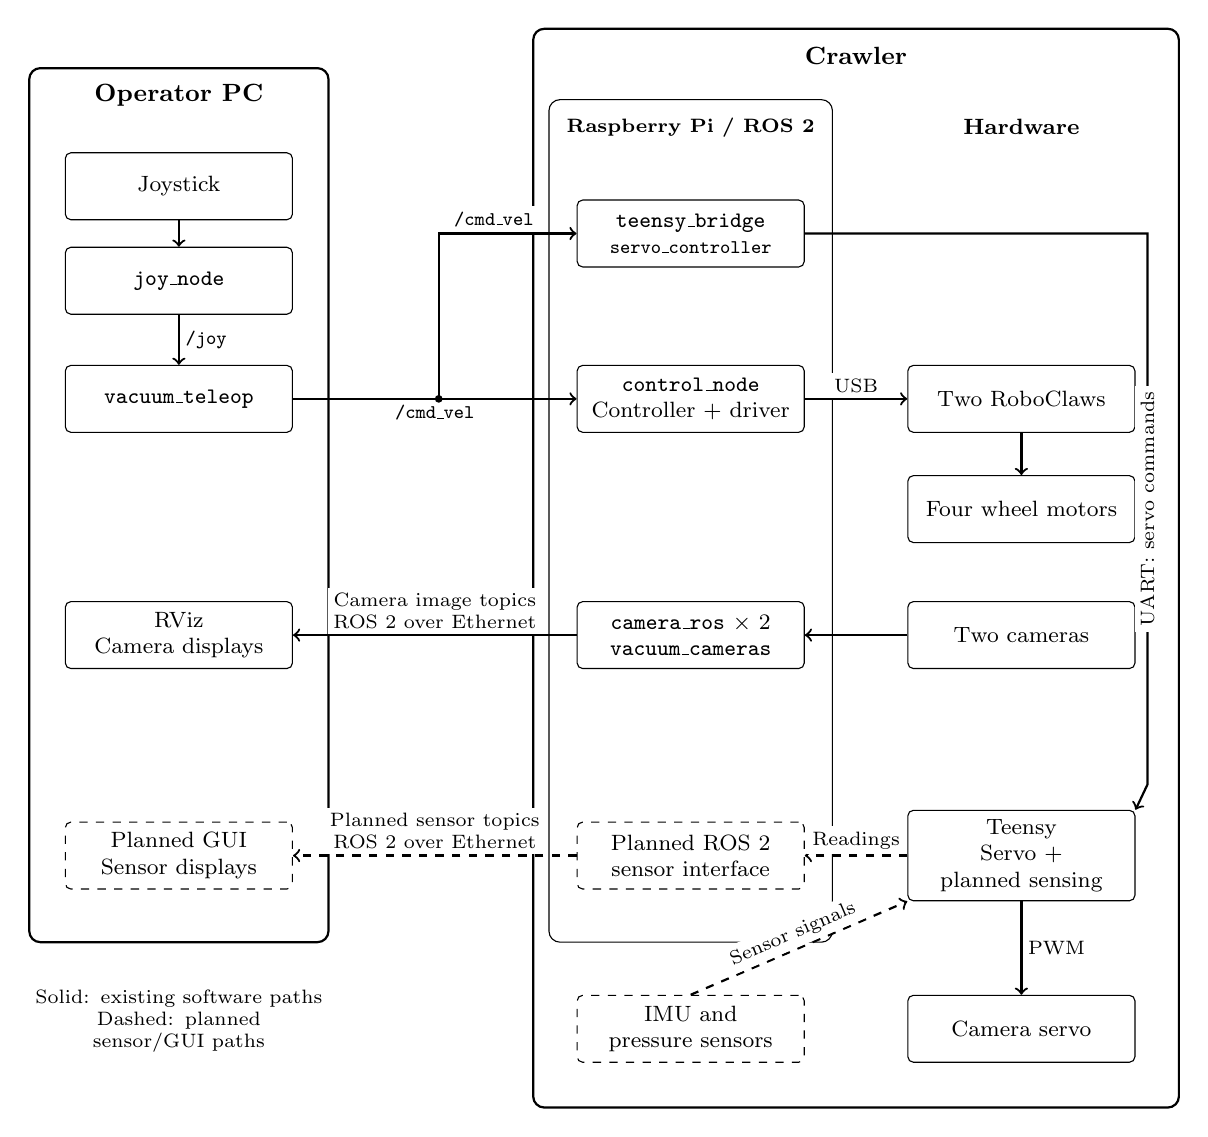
\begin{tikzpicture}[
  box/.style={draw, rounded corners=2pt, align=center, text width=2.65cm, minimum height=0.85cm, font=\footnotesize},
  link/.style={->, thick},
  planned/.style={->, thick, dashed},
  lab/.style={font=\scriptsize, align=center, fill=white, inner sep=2pt}]
% Deployment boundaries: ROS processes on the PC and Pi; hardware on the crawler.
\draw[rounded corners, thick] (-0.2,1) rectangle (3.6,-10.1);
\node[font=\small\bfseries] at (1.7,0.65) {Operator PC};
\draw[rounded corners, thick] (6.2,1.5) rectangle (14.4,-12.2);
\node[font=\small\bfseries] at (10.3,1.15) {Crawler};
\draw[rounded corners] (6.4,0.6) rectangle (10,-10.1);
\node[font=\scriptsize\bfseries] at (8.2,0.25) {Raspberry Pi / ROS 2};
\node[font=\footnotesize\bfseries] at (12.4,0.25) {Hardware};
\node[box] (joydev) at (1.7,-0.5) {Joystick};
\node[box] (joy) at (1.7,-1.7) {\texttt{joy\_node}};
\node[box] (teleop) at (1.7,-3.2) {\texttt{vacuum\_teleop}};
\node[box] (rviz) at (1.7,-6.2) {RViz\\Camera displays};
\node[box,dashed] (gui) at (1.7,-9) {Planned GUI\\Sensor displays};
\node[box] (bridge) at (8.2,-1.1) {\texttt{teensy\_bridge}\\{\scriptsize\texttt{servo\_controller}}};
\node[box] (drive) at (8.2,-3.2) {\texttt{control\_node}\\Controller + driver};
\node[box] (camera) at (8.2,-6.2) {\texttt{camera\_ros} $\times$ 2\\\texttt{vacuum\_cameras}};
\node[box,dashed] (sensing) at (8.2,-9) {Planned ROS 2\\sensor interface};
\node[box] (roboclaw) at (12.4,-3.2) {Two RoboClaws};
\node[box] (wheels) at (12.4,-4.6) {Four wheel motors};
\node[box] (cams) at (12.4,-6.2) {Two cameras};
\node[box] (teensy) at (12.4,-9) {Teensy\\Servo + planned sensing};
\node[box] (servo) at (12.4,-11.2) {Camera servo};
\node[box,dashed] (sensors) at (8.2,-11.2) {IMU and\\pressure sensors};
\draw[link] (joydev) -- (joy);
\draw[link] (joy) -- node[lab,right]{\texttt{/joy}} (teleop);
\draw[link] (teleop) -- node[lab,below]{\texttt{/cmd\_vel}} (drive);
\draw[link] (5,-3.2) |- node[lab,pos=0.7,above]{\texttt{/cmd\_vel}} (bridge);
\fill (5,-3.2) circle (1.4pt);
\draw[link] (drive) -- node[lab,above]{USB} (roboclaw);
\draw[link] (roboclaw) -- (wheels);
\draw[link] (cams) -- (camera);
\draw[link] (camera) -- node[lab,above]{Camera image topics\\ROS 2 over Ethernet} (rviz);
\draw[link] (bridge.east) -- (14,-1.1) -- node[lab,rotate=90]{UART: servo commands} (14,-8.1) -- (teensy.north east);
\draw[planned] (teensy) -- node[lab,above]{Readings} (sensing);
\draw[planned] (sensing) -- node[lab,above]{Planned sensor topics\\ROS 2 over Ethernet} (gui);
\draw[planned] (sensors.north) -- node[lab,above,sloped]{Sensor signals} (teensy.south west);
\draw[link] (teensy) -- node[lab,right]{PWM} (servo);
\node[lab,text width=3.7cm] at (1.7,-11.1) {Solid: existing software paths\\Dashed: planned sensor/GUI paths};
\end{tikzpicture}
\caption[ROS 2 architecture across the operator PC and crawler]{ROS 2 architecture showing the operator PC, Raspberry Pi processes, and crawler hardware. The PC sends movement and servo commands and receives camera images over Ethernet. Planned sensor readings pass through the Teensy to a ROS 2 interface and the GUI. Software paths do not imply completed hardware validation.}
\label{fig:control-communications}
\end{figure}
\clearpage
\section{Drive Control}
\label{sec:drive-control}
The drive implementation separates joystick interpretation, command calculation, and motor-controller communication. Four wheel motors are connected through two RoboClaw controllers, assigned to the front and rear pairs. Although the four channels are separately addressable, the software commands the two motors on each side together. The package named \texttt{vacuum\_controller} controls crawler travel; it does not implement pneumatic vacuum regulation \citep{hernandezVacuumCrawler2026}.

\subsection{Joystick Input and Teleoperation}
\label{sec:joystick-teleoperation}
The standard \texttt{joy\_node} reads the controller and publishes joystick inputs on \texttt{/joy} \citep{rosJoyDriver}. The project's \texttt{vacuum\_teleop\_node} converts these inputs into forward, turning, and camera-servo commands on \texttt{/cmd\_vel}. The wheel controller uses the forward and turning fields, while the Teensy bridge reads the servo command carried in \texttt{angular.x}. This shared message lets the operator control travel and camera direction from the same joystick \citep{hernandezVacuumCrawler2026}.
\subsection{Wheel Command Calculation and Motor Driver}
\label{sec:wheel-control-driver}
The \texttt{control\_node} receives movement commands and updates the motor outputs at a nominal 20~Hz. The \texttt{VacuumController} class combines forward and turning demands into left- and right-side commands. When a demand exceeds the configured 25\% duty limit, both sides are reduced proportionally to preserve the requested steering balance. The \texttt{VacuumDriver} class sends these commands through Universal Serial Bus (USB) serial connections to the front and rear RoboClaw controllers and checks their replies. Each controller drives one right wheel on M1 and one left wheel on M2 \citep{hernandezVacuumCrawler2026}.

This implementation uses open-loop motor duty control, without encoder feedback or speed regulation. Its example wheel separation and speed scale still require calibration to the assembled crawler; commanded velocity should therefore not be interpreted as measured travel speed.
\subsection{Teensy Bridge and Camera Servo}
\label{sec:teensy-servo}
The \texttt{servo\_controller} package supplies the \texttt{teensy\_bridge} node and Teensy firmware. The bridge subscribes to \texttt{/cmd\_vel}, extracts \texttt{angular.x}, and divides it by 10 to recover the joystick demand. It clamps that demand to $[-1,1]$, applies a 5\% deadband, and maps the remaining input to a maximum commanded servo rate of 20 degrees per second. This provides camera-direction commands alongside crawler travel commands \citep{hernandezVacuumCrawler2026}.

The intended connection uses the Raspberry Pi's universal asynchronous receiver/transmitter (UART) interface and Teensy \texttt{Serial1} at 115200 baud. The bridge verifies a firmware identification response before sending movement commands. The firmware integrates the requested angular rate, constrains the commanded position to 60--150 degrees, and drives pin 4 using the external \texttt{PWMServo} library. Pulse-width modulation (PWM) remains enabled while holding position. Output is initially disabled; the first valid speed command applies the inherited 149-degree starting position, including when the requested speed is zero.

The repository identifies the pin assignment, angular limits, and starting angle as recovered from an earlier sketch. The new bridge and firmware add identification, nonblocking parsing, and elapsed-time position updates around those inherited settings. Physical validation of the servo connection remains pending \citep{hernandezVacuumCrawler2026}.

\subsection{Command Timeouts and Fault Handling}
\label{sec:control-faults}
% Placeholder: complete after the operating behavior and validation are documented.
\section{Sensor Feedback}
\label{sec:sensor-camera}
Sensor feedback is intended to give the operator visual, attitude, and pneumatic-state information. The repository implements the image-stream path, while IMU and pressure interfaces remain to be documented. No sensor-based correction of wheel commands is implemented at the reviewed revision.

\subsection{3D Camera Stream}
\label{sec:camera-stream}
The intended 3D camera function currently has a dual-image-stream implementation. The \texttt{vacuum\_cameras} package launches two instances of the external \texttt{camera\_ros} driver, which obtains images through \texttt{libcamera} and exposes ROS image and camera-information topics \citep{cameraRosDriver}. Project documentation identifies two IMX219 camera modules on the Raspberry Pi and explicitly states that they are neither synchronized nor stereo calibrated. The available implementation therefore supports two-dimensional viewing; it does not establish a depth stream, point cloud, or metric 3D measurements \citep{hernandezVacuumCrawler2026}.

The launch file places the nodes in separate namespaces, \texttt{/cameras/camera0} and \texttt{/cameras/camera1}. Each publishes \texttt{image\_raw}, \texttt{image\_raw/compressed}, and \texttt{camera\_info}. Requested settings are 320 by 240 pixels, a 100000-microsecond frame duration corresponding to 10 frames per second, and Joint Photographic Experts Group (JPEG) quality 60 for compressed images. These are settings rather than guaranteed delivered rates. Camera-information messages alone do not demonstrate calibration; the project documentation identifies the intrinsics as uncalibrated until calibration data are supplied.

The RViz preview uses two compressed-image displays with best-effort reliability and a queue depth of one. Best-effort delivery permits sample loss; the queue limits retained history \citep{ros2JazzyQoS}. This configuration is intended to favor recent viewing information. Its effect on visible delay and image continuity must be measured under the intended network and processing load.

The camera wrapper selects locally built, revision-pinned \texttt{libcamera} and \texttt{camera\_ros} dependencies to address the documented Raspberry Pi compatibility issue. These remain external drivers; the project package supplies build configuration, launch settings, and stream checks. Completing the 3D function requires identification of the depth-producing hardware or stereo-processing path, calibration, coordinate frames, and evidence of usable depth output. Those functions are not inferred from the presence of two cameras.

\subsection{IMU}
\label{sec:imu-feedback}
\draftnote{Placeholder. Identify the IMU model, mounting orientation, interface, ROS 2 driver and topic, calibration, and intended feedback. No IMU acquisition or fusion implementation was found in the reviewed repository.}

\subsection{Pressure Sensors}
\label{sec:pressure-feedback}
The pressure sensors will connect to the Teensy for acquisition and transmission to ROS 2. Pressure feedback is planned to relate the pneumatic operating condition to the vacuum system described in Chapter~\ref{chap:vacuum}. Acquisition must distinguish compressed-air supply pressure from suction or differential pressure and identify each measurement location. The repository contains no pressure-sensor driver, channel map, calibration, or publishing node, so it does not establish installed models, measurement ranges, or live pressure telemetry.

A proposed ROS interface is \texttt{sensor\_msgs/msg/FluidPressure}, which defines absolute pressure in pascals together with measurement time, sensor frame, and variance \citep{rosFluidPressureMessage}. Gauge or differential readings must not be presented as absolute pressure without the appropriate reference or conversion. Once the transducers and acquisition hardware are confirmed, the implementation should document raw-reading conversion, the zero/reference procedure, sampling rate, and treatment of disconnected or invalid inputs. Pressure-based alarms and automatic regulation remain proposed functions until their logic and response are implemented and tested.

\section{Graphical User Interface}
\label{sec:operator-interface}
\draftnote{Placeholder for the graphical user interface (GUI). Document the final layout, camera displays, commands, sensor readings, and connection/fault indications after implementation. The repository's RViz camera preset is a viewing aid, not evidence of a completed custom GUI.}
